% !TEX encoding = UTF-8 Unicode
%!TEX root = ../Main/thesis.tex
% !TEX spellcheck = en-US
%%=========================================
\documentclass[../Main/thesis.tex]{subfiles}
\begin{document}
\chapter{Third Iteration - Second prototype}
\label{ch:development-2}
This chapter describes the third, and final, iteration of the development process.
In this iteration the prototypes from Chapter~\ref{ch:development-1} improved and tested.

\section{Android application}
The Android application went through some changes in this iteration.
The most visible change is a new design for the app.
Some of the design changes are shown in Figure~\ref{fig:new-design}.
It was redesigned to be more user friendly and consistent with the design of the exercise management tool.

\begin{figure}[h]
	\centering
	\begin{subfigure}{0.2\textwidth}
		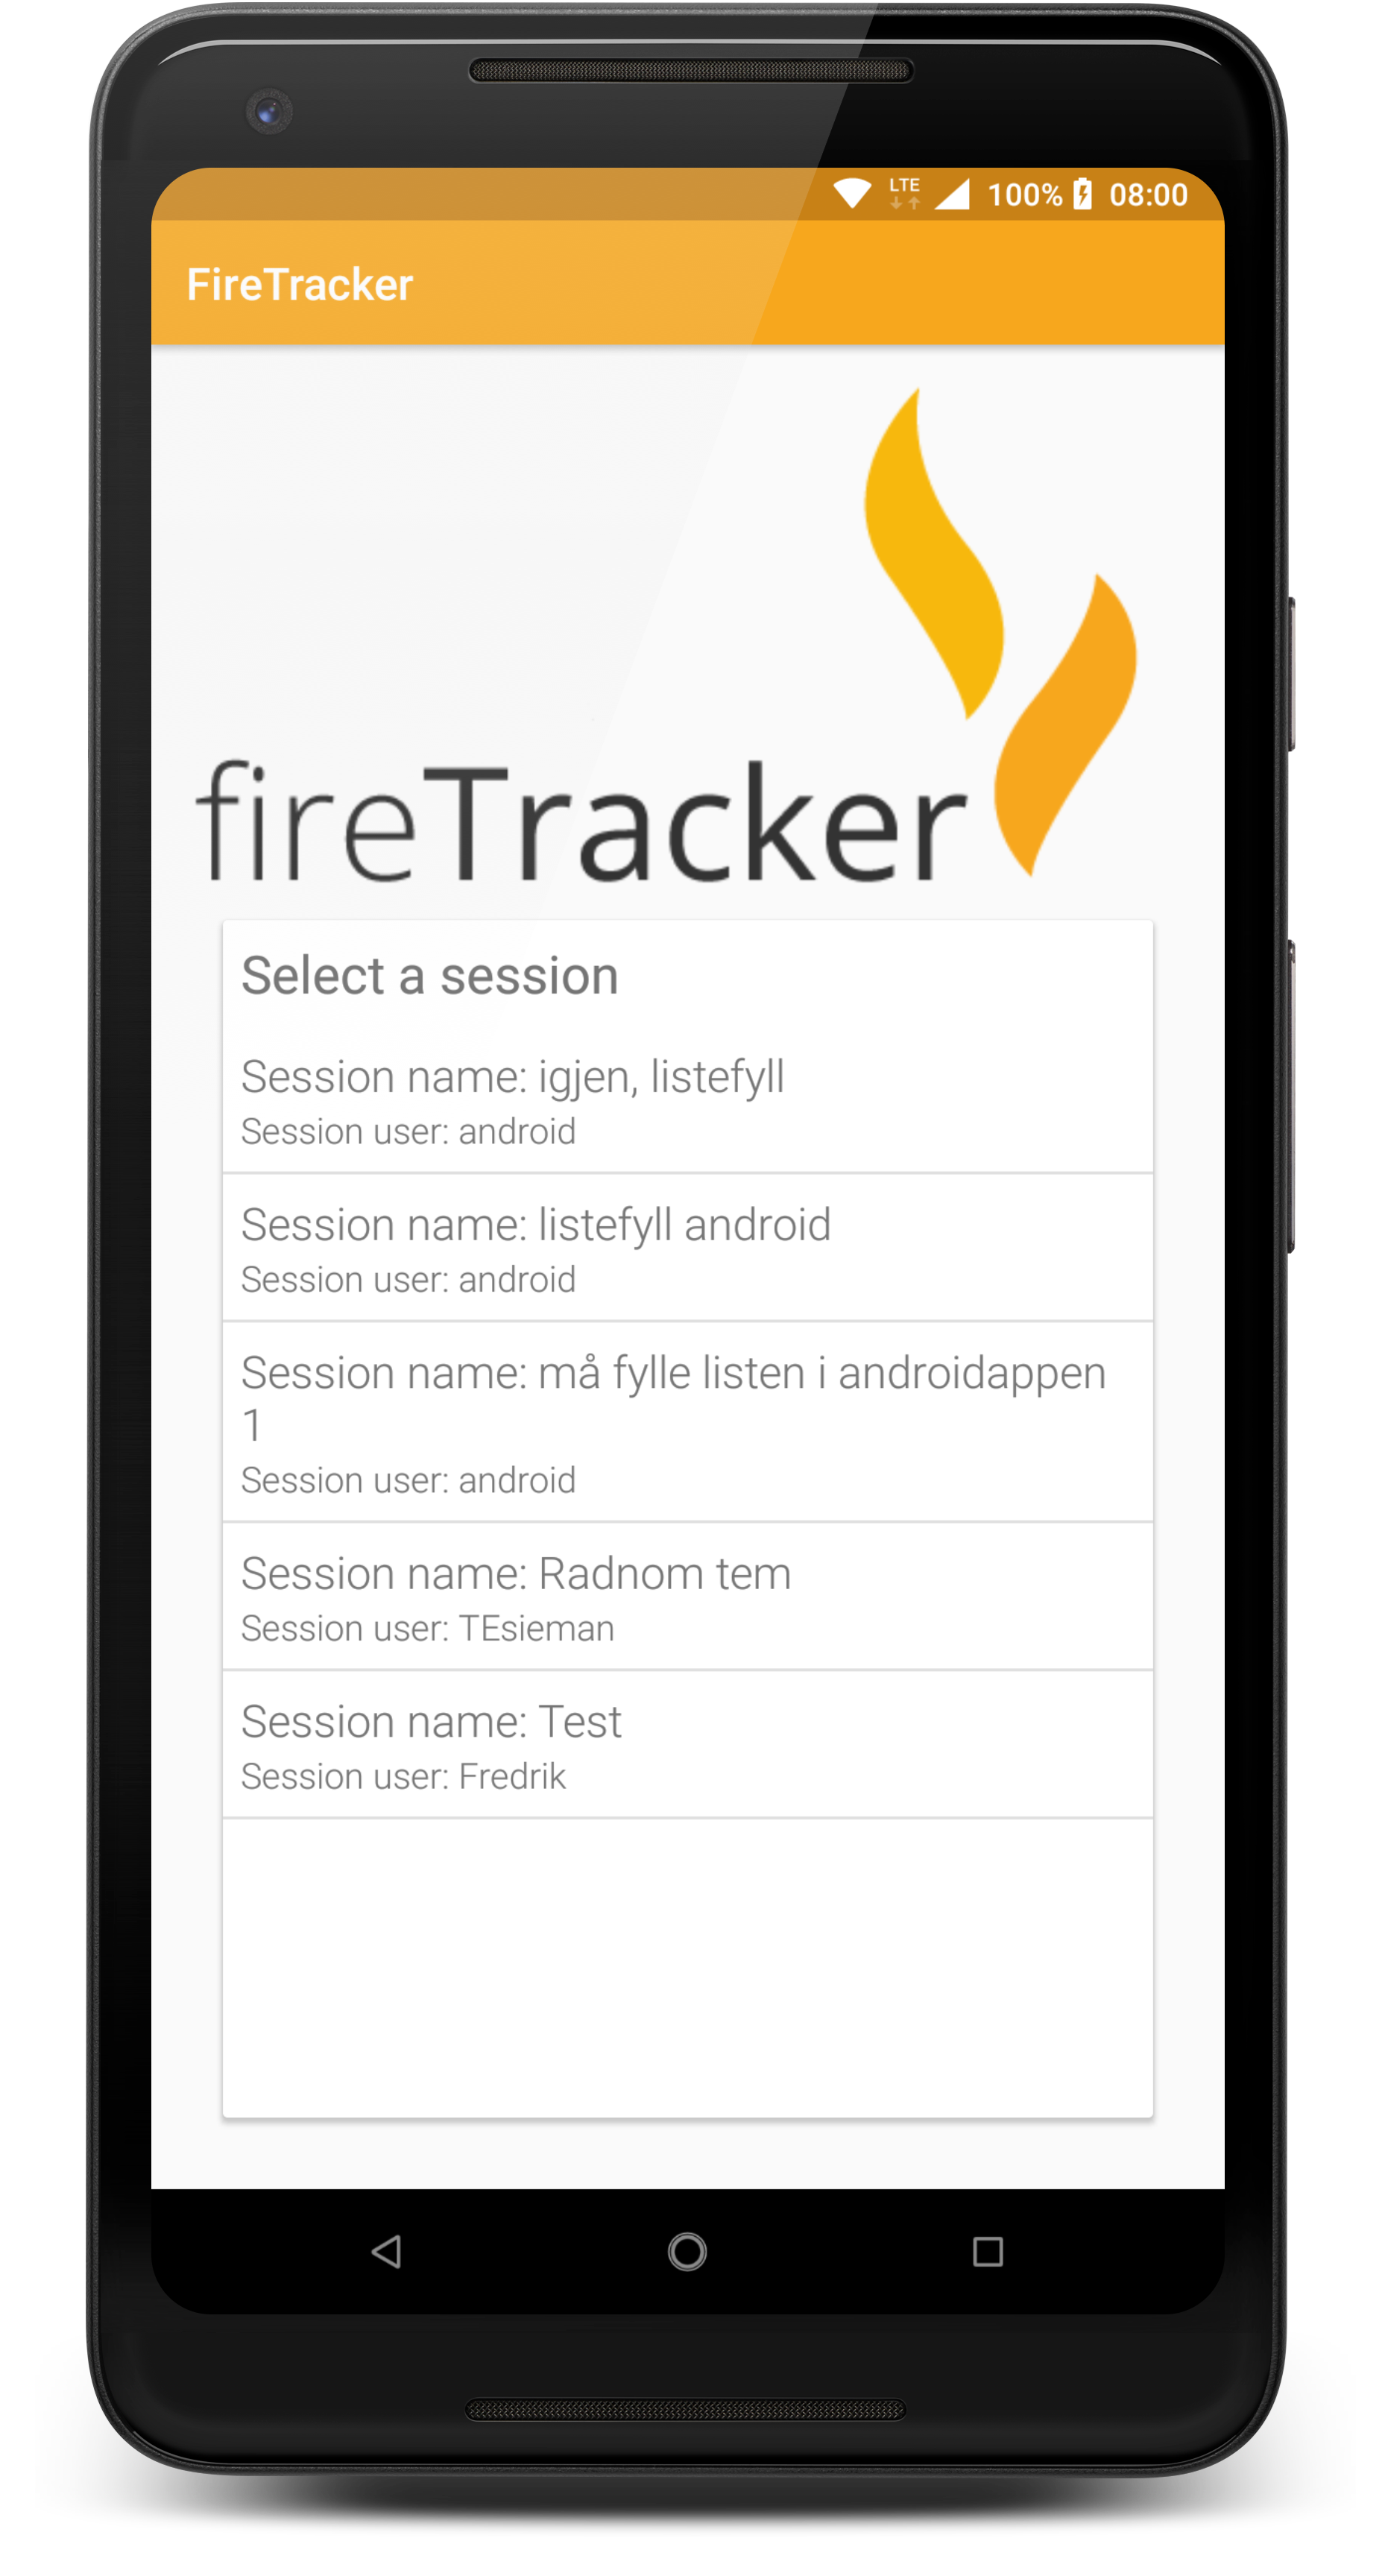
\includegraphics[width=\textwidth]{../fig/firetracker_app_old_1}
		\caption{Old design}
		\label{fig:app-old-design-sessionlist-iteration3}
	\end{subfigure}
	\begin{subfigure}{0.2\textwidth}
		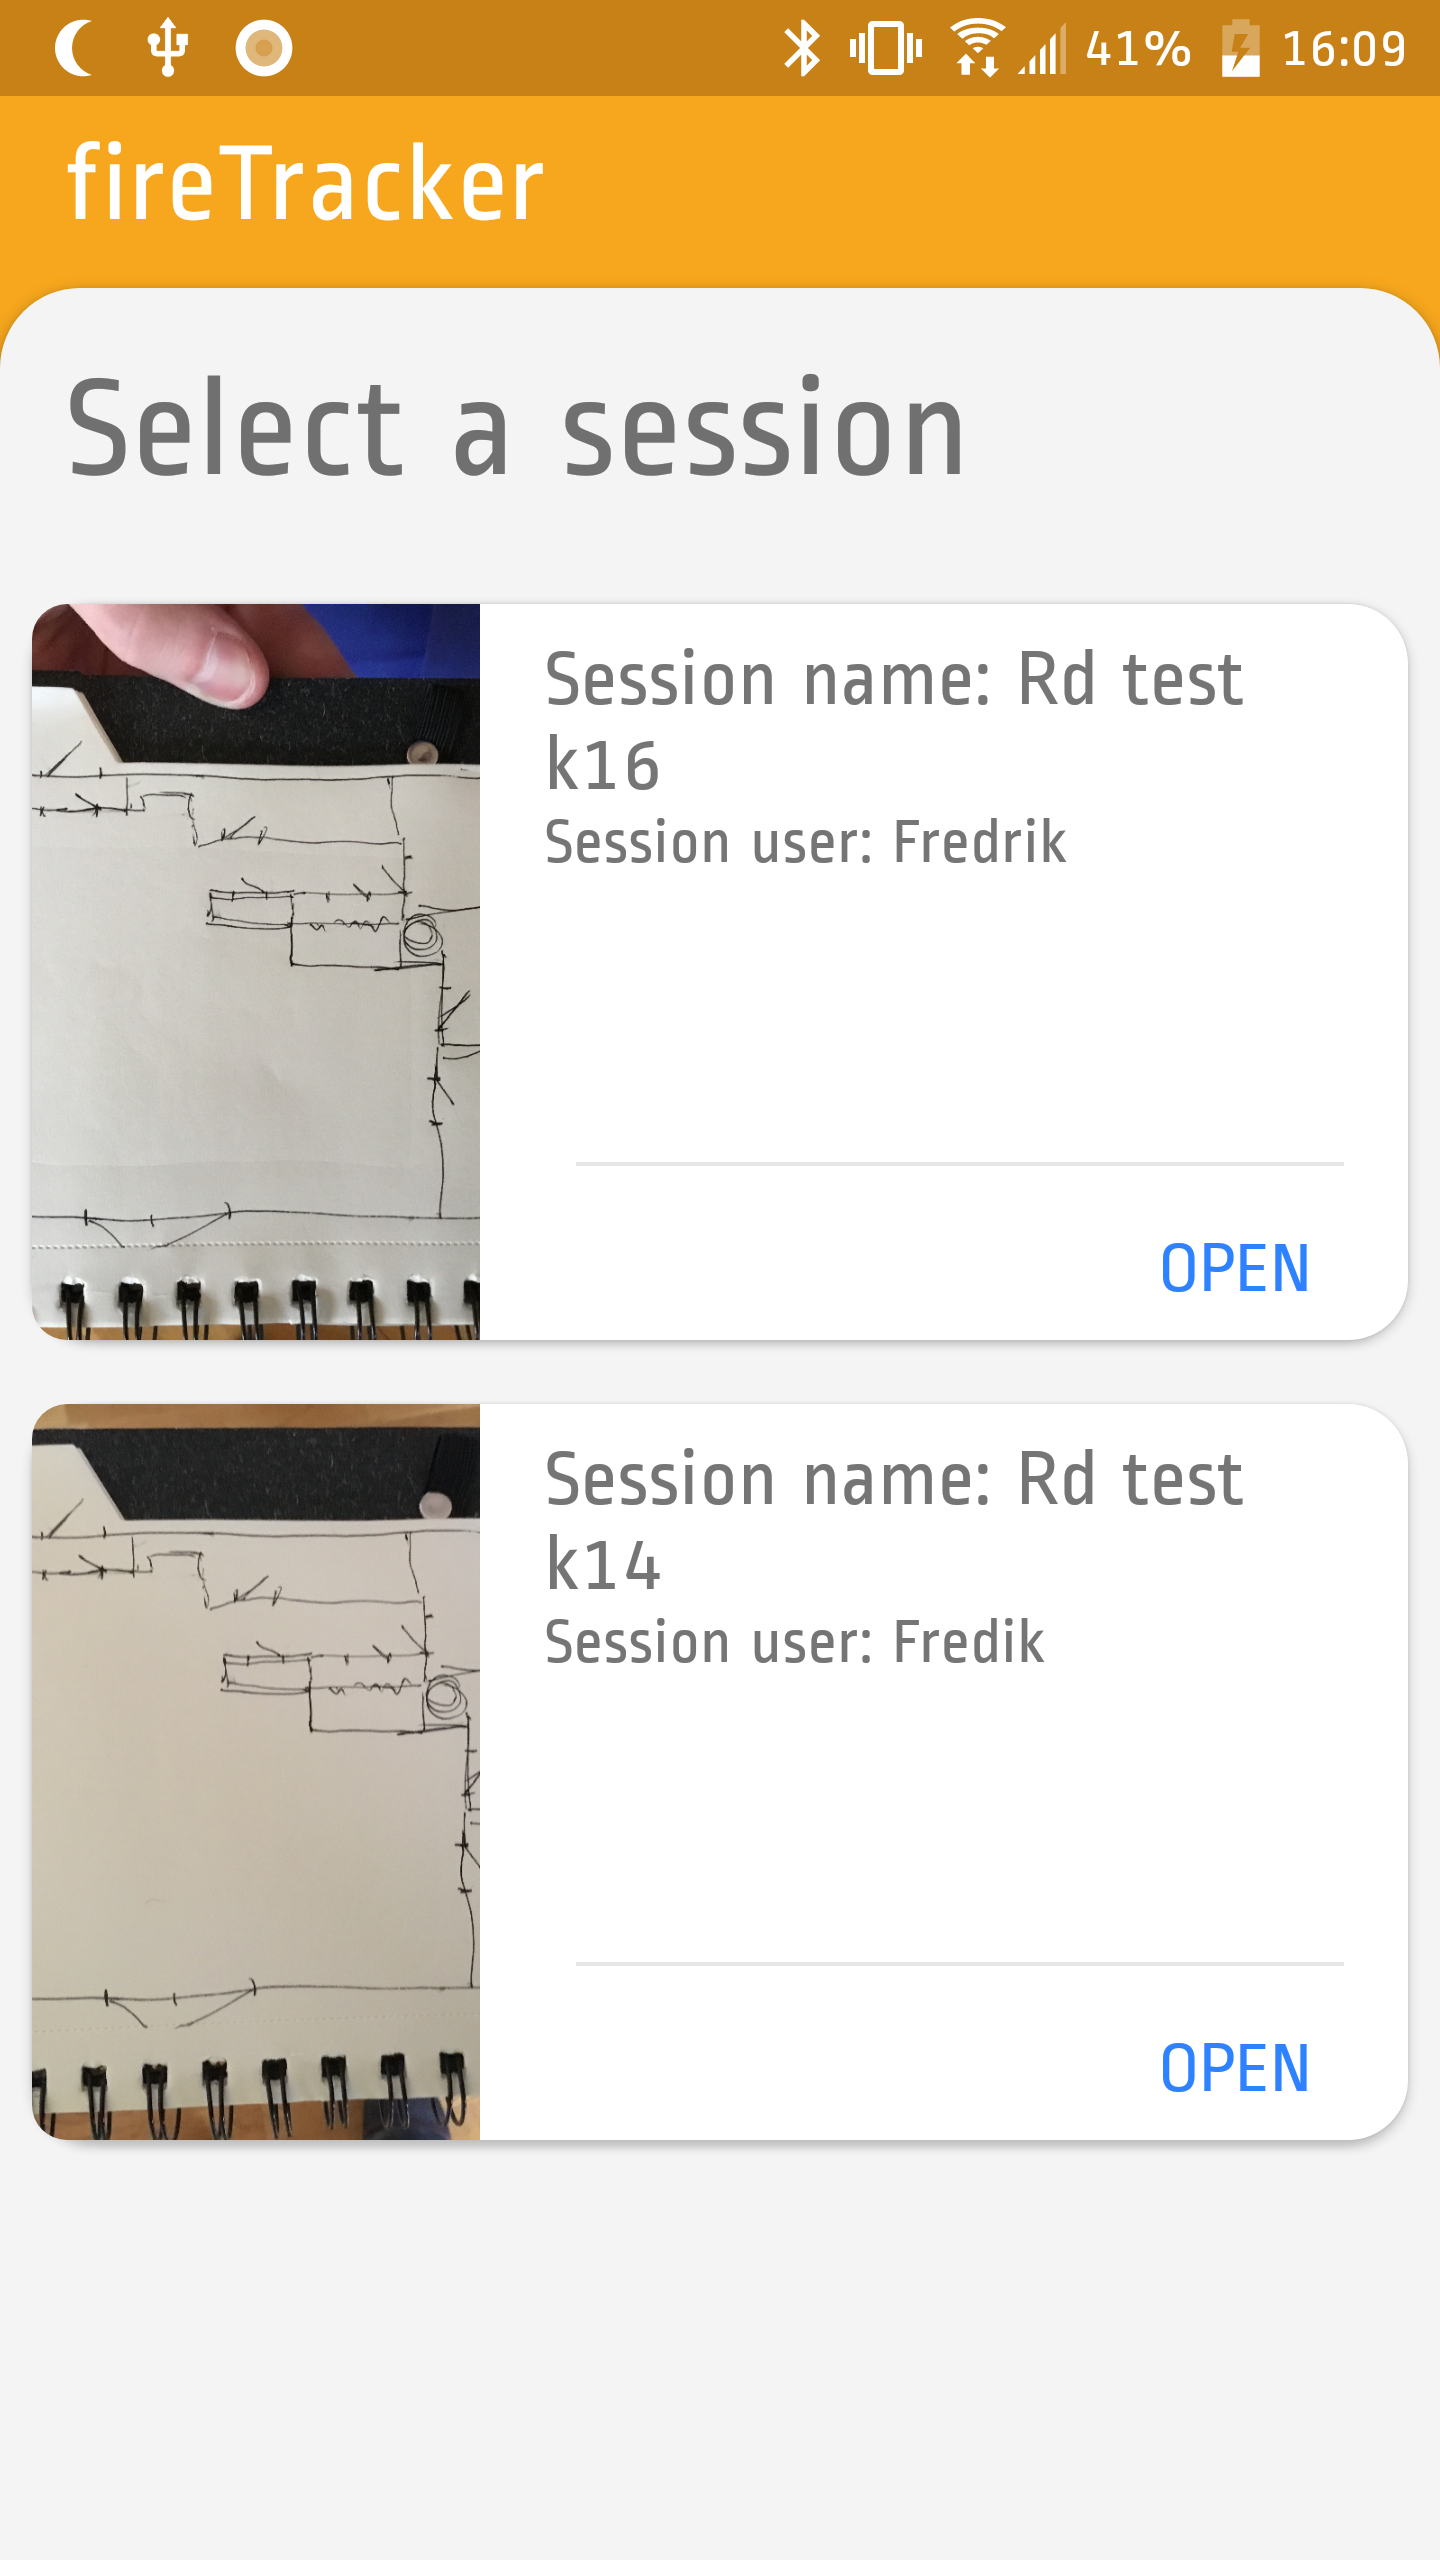
\includegraphics[width=\textwidth]{../fig/firetracker_app_new_1}
		\caption{New design}
		\label{fig:app-new-design-sessionlist-iteration3}
	\end{subfigure}
	\begin{subfigure}{0.2\textwidth}
		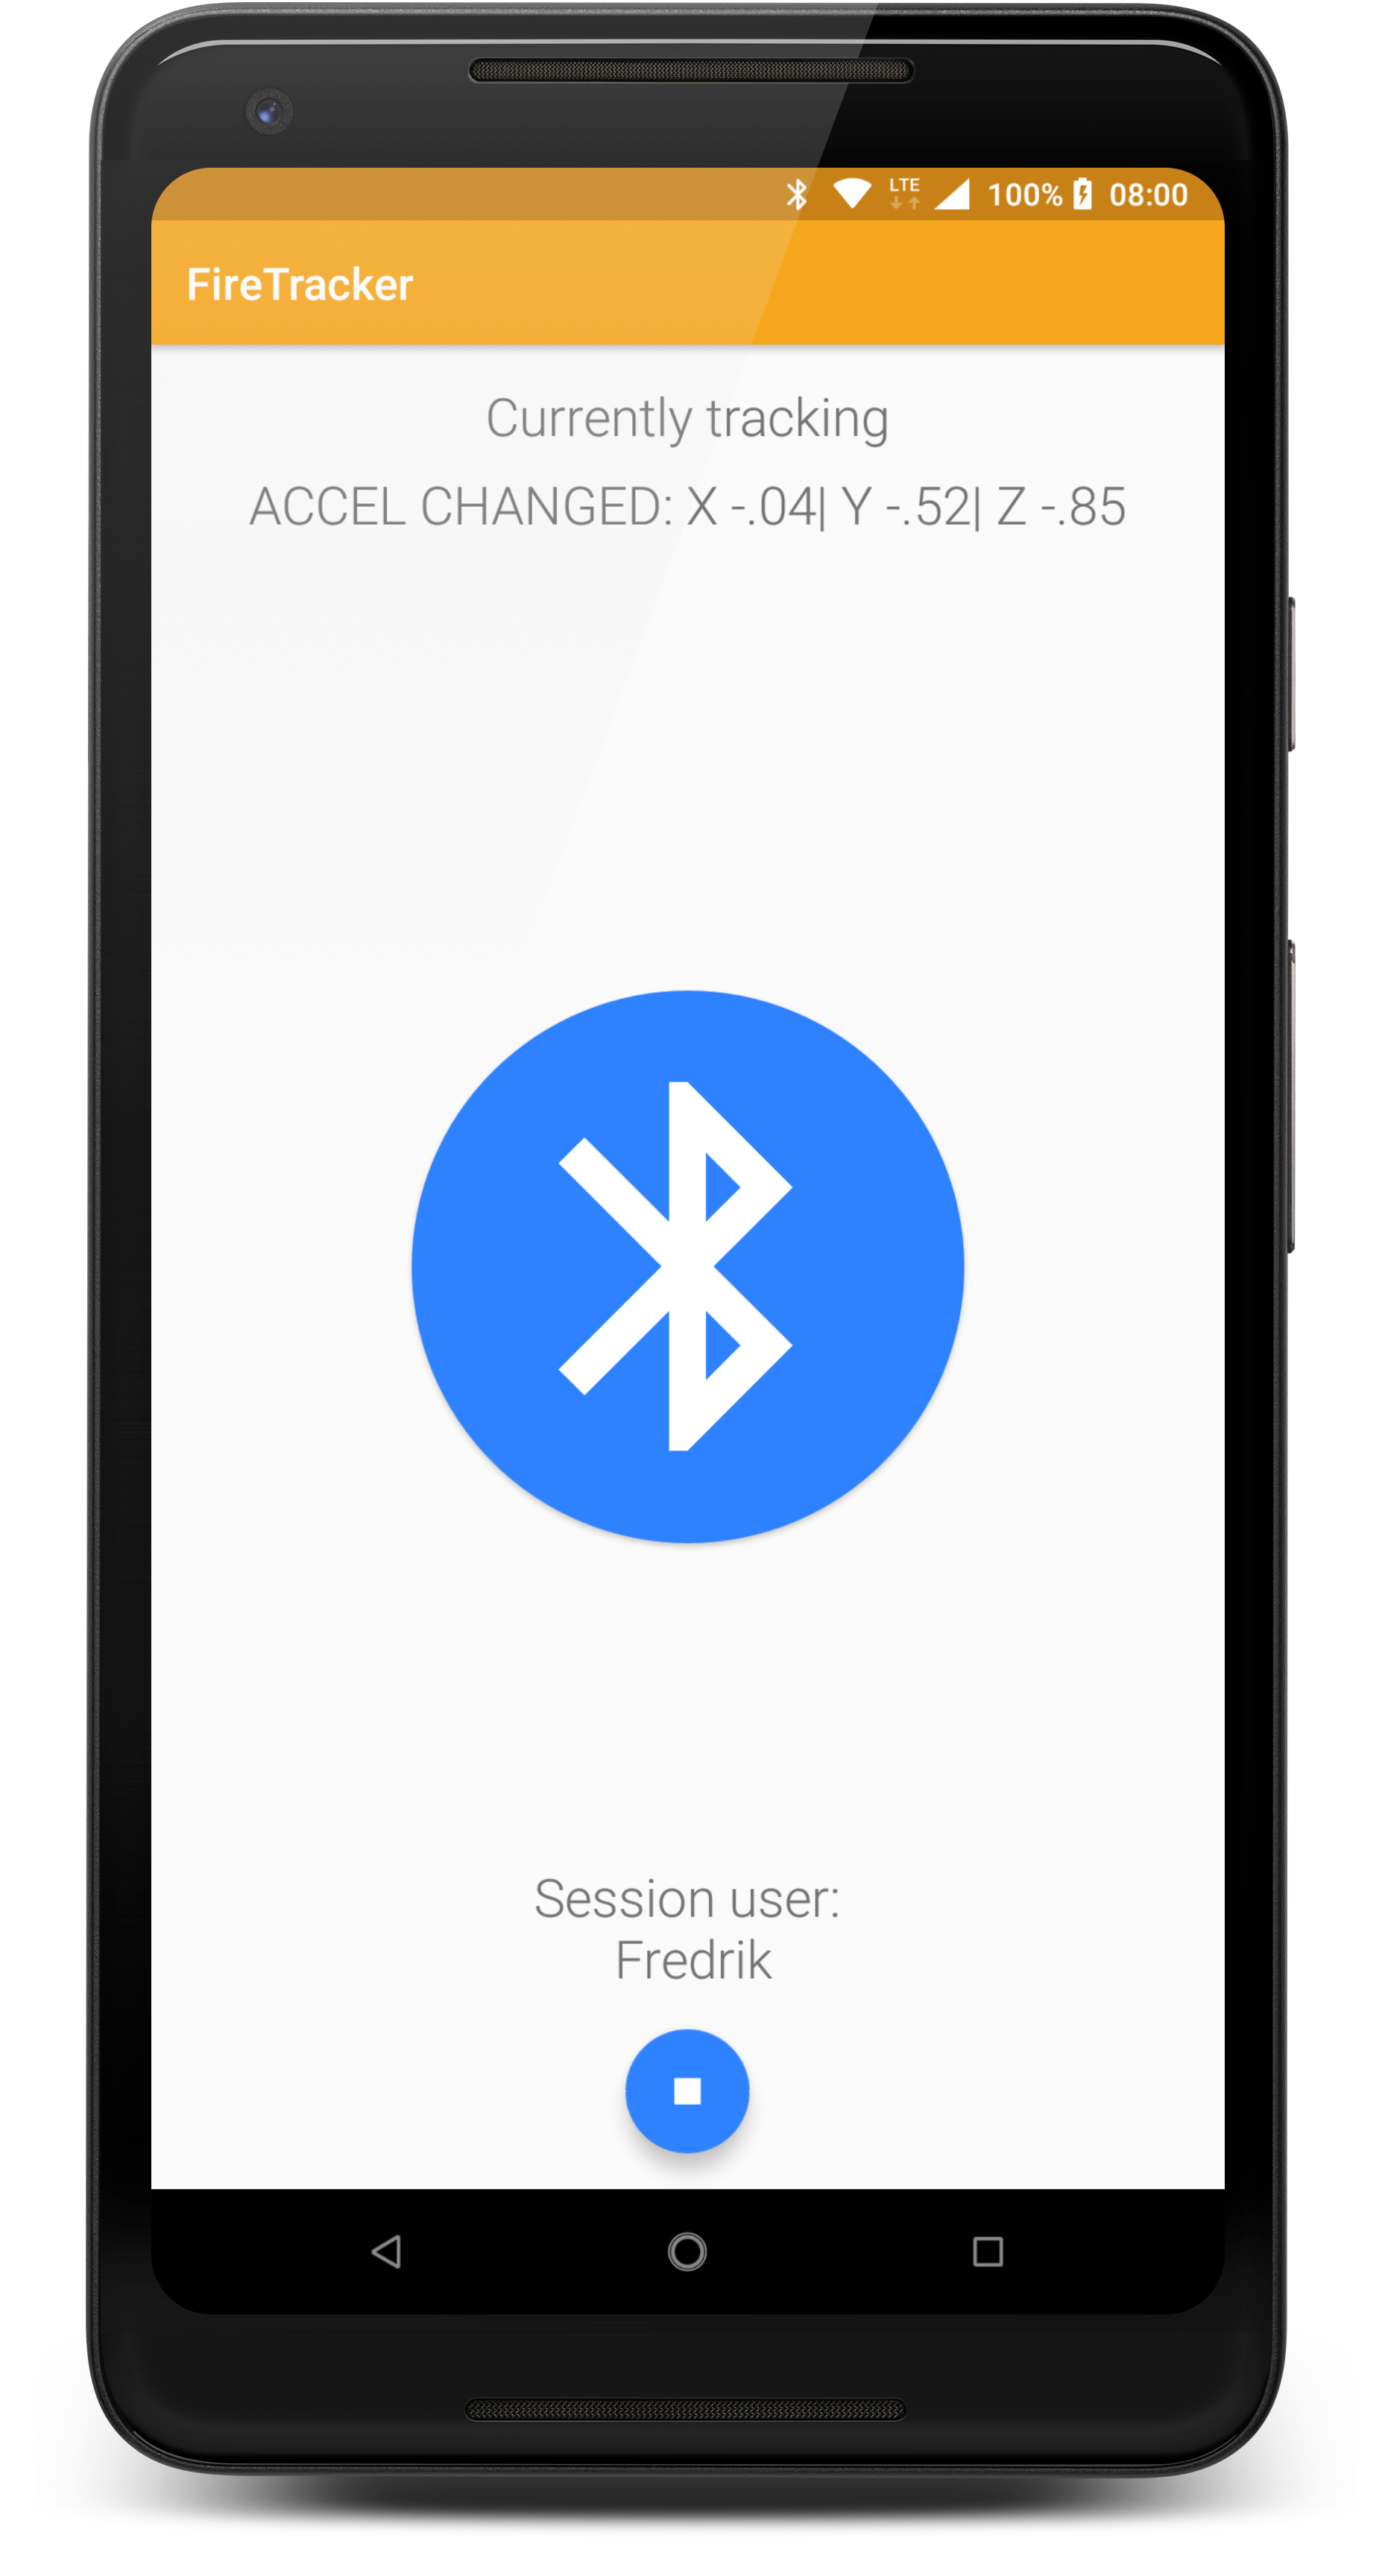
\includegraphics[width=\textwidth]{../fig/firetracker_app_old_3}
		\caption{Old design}
		\label{fig:app-old-design-tracking-iteration3}
	\end{subfigure}
	\begin{subfigure}{0.2\textwidth}
		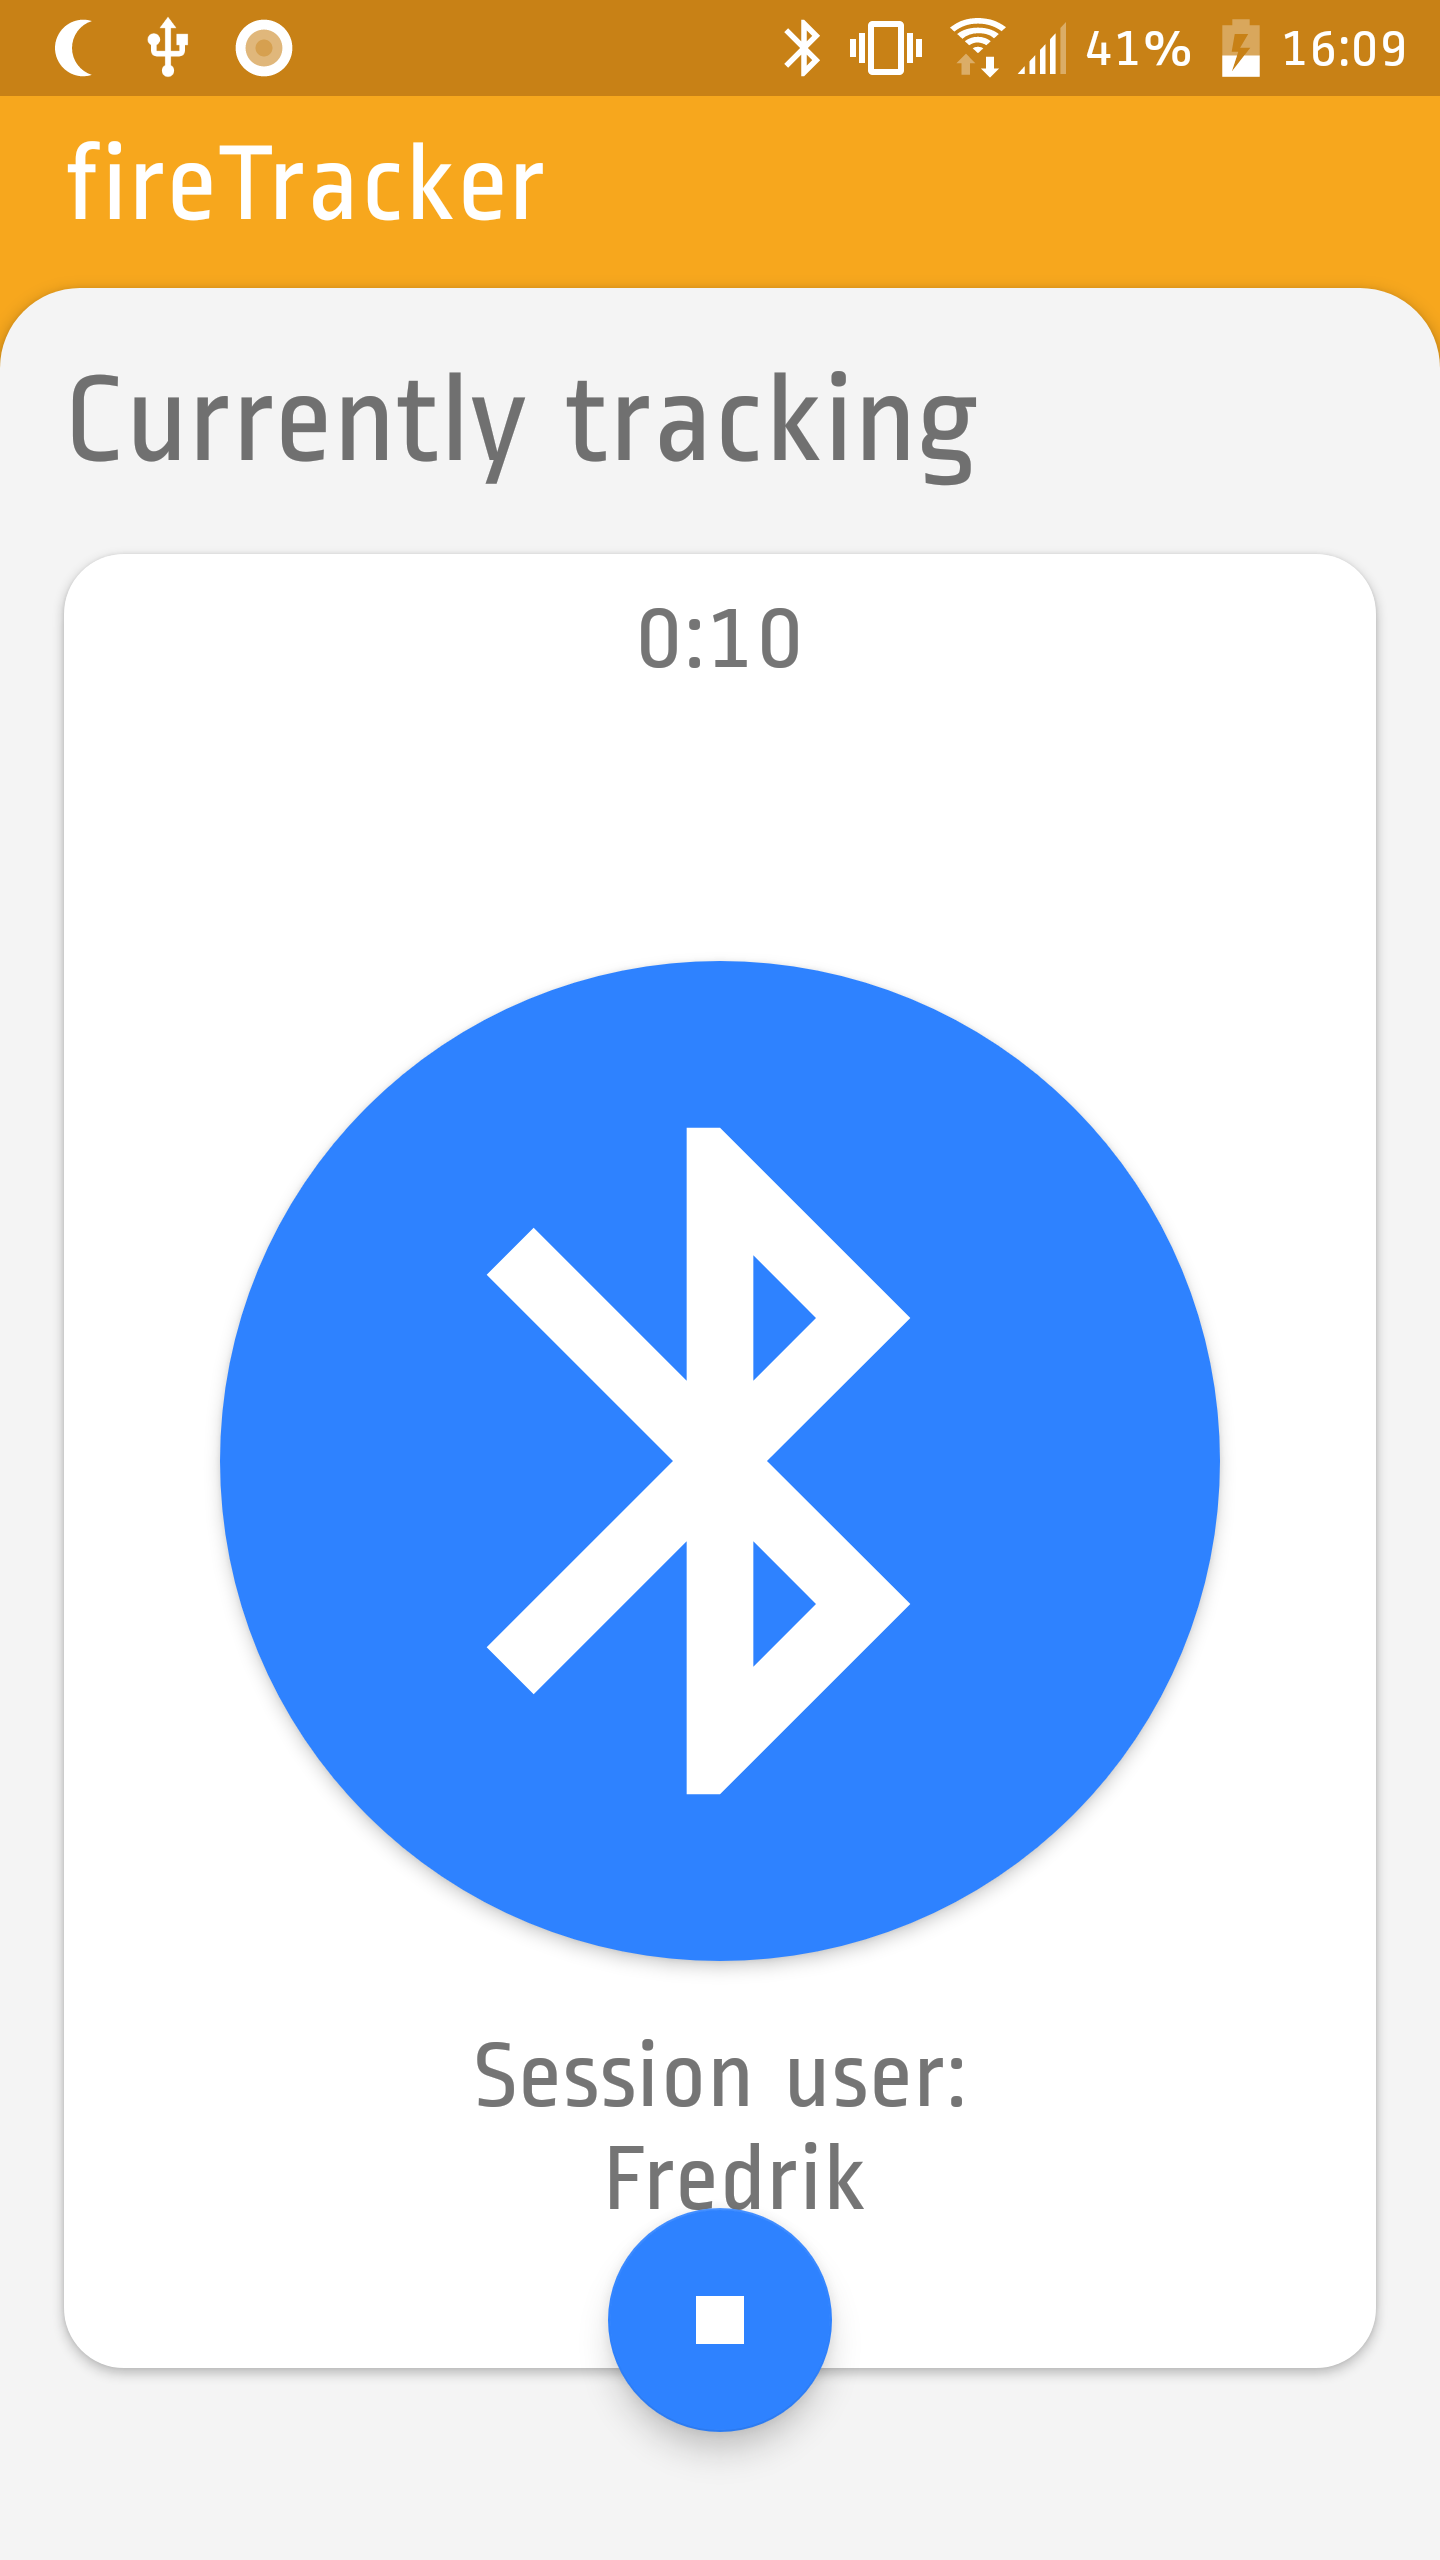
\includegraphics[width=\textwidth]{../fig/firetracker_app_new_2}
		\caption{New design}
		\label{fig:app-new-design-tracking-iteration3}
	\end{subfigure}
	\caption[Design changes in Android application]{Design changes in Android application. List of sessions screen (left) and tracking activity (right)}
	\label{fig:app-first-prototype}
\end{figure}
\todo{fix images}

As the fire department would prefer to have the system in Norwegian the app was translated into both Nynorsk and Bokmål.
The app will use the language which is set as default in the phone settings.
A safety feature was also added to prevent loss of data.
If the app is unable to upload data from a session for some reason, the user is given the opportunity to save the session locally on the device for later uploading.
This way the exercise can continue and the device can be used for another session immediately. 

On the tracking screen a timer was added to make it easier to see how long the session has lasted.
The settings for how often the phone should search for BLE signals was also changed to the shortest possible interval.

\section{Back end}
During this iteration there improvements were made to the back-end, both to the web-server part and to the data processing part.
Those changes are described in the following sections.

\subsection{Web-server}
An endpoint for deleting beacons from the database was added to the web-server during this iteration.
The other endpoints were restructured removing the ``raw''-part of the session related URLs.
Instead of specifying if the session should be unprocessed or not the default is to return processed locations if they exists, but not return all the collected data associated with a session.
This was done to reduce the amount of data that is returned, which effected the loading time of large sessions.
If one wants all the data points for a session it is possible to specify that.
When getting a list of sessions the default is to exclude both locations and data points.
All available endpoints with their description is presented in Table~\ref{tab:endpoints-2}.

\begin{table}[]
\caption{Web-server endpoints after the third iteration}
\begin{tabular}{|p{0.2\linewidth}|p{0.15\linewidth}|p{0.15\linewidth}|p{0.4\linewidth}|}
\hline
\textbf{Relative path} & \textbf{Request Type} & \textbf{Parameters} & \textbf{Description}                                        \\ \hline
/session               & OPTIONS               &                     & Create a new session                                        \\ \hline
/sessions              & GET                   &                     & Get all sessions                                            \\ \hline
/sessions              & POST                  & Finished            & Get sessions where the finished-flag is set to ``Finished'' \\ \hline
/session:id            & GET                   &                     & Get a session with the ID ``id''                            \\ \hline
/fullsession:id        & GET                   &                     & Get a session with the ID ``id'' including datapoints       \\ \hline
/session:id            & PUT                   &                     & Update a session with the ID ``id''                         \\ \hline
/beacon                & OPTIONS               &                     & Create a new beacon                                         \\ \hline
/beacon/delete         & POST                  & Id                  & Delete the beacon with the ID ``id''                        \\ \hline
/beacons               & GET                   &                     & Get a list of all beacons                                   \\ \hline
/sessionbeacon         & POST                  &                     & Create a new beacon for a spesific session                  \\ \hline
/map                   & POST                  &                     & Upload a map                                                \\ \hline
\end{tabular}
\label{tab:endpoints-2}
\end{table}

\subsection{Data processing}
The data processing algorithm went through a massive overhaul in this iteration.
The estimation of mid-points between two locations was removed, and 
\todo{Finish this}

\section{Data specifications}
There were some minor changes to the data specifications in this iteration.
To visualize the time the smoke divers use in each location better it was decided to add the time they arrive and leave each location, in addition to the duration of the stay.
This change can be seen in Source~Code~\ref{listing:location-json-iteration3}.

\begin{figure}[h]
\begin{minipage}{0.45\textwidth}
\centering
\begin{minted}
	[
	frame=lines,
	linenos
	]{json}
{
  "ID": <integer>,
  "SessionId": <integer>,
  "XCoordinate": <float>,
  "YCoordinate": <float>,
  "Duration": <integer>,
  "Walking": <boolean>,
  "HeadMovement": <boolean>
}
\end{minted}
%\captionof{listing}{Old location JSON-object}
%\label{listing:location-json-2}
\end{minipage}
\hfill
\begin{minipage}{0.45\textwidth}
\centering
\begin{minted}
	[
	frame=lines,
	linenos
	]{json}
{
  "ID": <integer>,
  "SessionId": <integer>,
  "StartTime": <integer>,
  "EndTime": <integer>,
  "XCoordinate": <float>,
  "YCoordinate": <float>,
  "Duration": <integer>,
  "Walking": <boolean>,
  "HeadMovement": <boolean>
}
\end{minted}
%\captionof{listing}{New location JSON-object}
%\label{listing:location-json-3}
\end{minipage}
\captionof{listing}{Updated Location JSON-object}
\label{listing:location-json-iteration3}
\end{figure}

\section{Testing}
\subsection{Beacon signal strength}

\end{document}
